\chapter{Исследовательская часть}

\section{Технические характеристики}
Технические характеристики устройства, на котором выполнялись
замеры по времени:

\begin{itemize}
    \item Процессор: Intel Core i7 9750H 2.6 ГГц;
    \item Оперативная память: 16 ГБ;
    \item Операционная система: Kubuntu 22.04.3 LTS x86\_64 Kernel: 6.2.0-36-generic
\end{itemize}

Во время проведения измерений времени ноутбук был подключен к сети электропитания и был нагружен только системными приложениями.

\section{Демонстрация работы программы}

На рисунке \ref{fig:img_prog} показан пример работы с программой.


\begin{figure}[ht!]
	\centering
	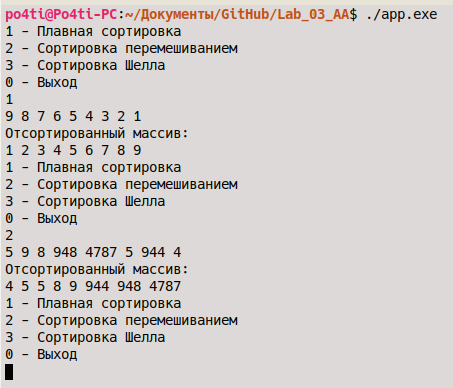
\includegraphics[width=170mm]{img/img_prog.png}
	\caption{Демонстрация работы программы.\label{overflow}}
	\label{fig:img_prog}
	\end{figure}


\clearpage

\section{Временные характеристики}


Исследование временных характеристик реализованных алгоритмов производилось на массивах размером 1 -- 500 с шагом 10.

\begin{figure}[ht!]
	\centering
	\includesvg[width=1.0\textwidth]{img/plotting_data1.svg}
	\caption{Результат измерений времени работы (в мс) алгоритмов сортировок на неотсортированных массивах\label{overflow}}
	\label{fig:plotting_data1}
	\end{figure}
\clearpage

\begin{figure}[ht!]
	\centering
	\includesvg[width=1.0\textwidth]{img/plotting_data2.svg}
	\caption{Результат измерений времени работы (в мс) алгоритмов сортировок на отсортированных массивах\label{overflow}}
	\label{fig:plotting_data2}
	\end{figure}

\begin{figure}[ht!]
	\centering
	\includesvg[width=1.0\textwidth]{img/plotting_data3.svg}
	\caption{Результат измерений времени работы (в мс) алгоритмов сортировок на отсортированных обратно массивах\label{overflow}}
	\label{fig:plotting_data3}
	\end{figure}

	
\section{Характеристики по памяти}

Пусть дан массив N элементов сравниваемого типа int. Тогда затраты по памяти для алгоритмов будут следующие:

\subsection*{Плавная сортировка}

Используемые переменные:
\begin{itemize}
	\item k первых чисел леонардо -- $k \cdot size(int)$
	\item переменные i, j, k в heapify -- $3 \cdot size(int)$
	\item переменные p q r в теле алгоритма -- $3 \cdot size(int)$
	\item массив -- $N \cdot size(int)$
	\item переменная-буфер для обмена элементов местами -- $1 \cdot size(int)$
\end{itemize}

Итого, для плавной сортировки:
\begin{equation}
M_{smooth} = k \cdot size(int) + 3 \cdot size(int) + 3 \cdot size(int) + N \cdot size(int) + 1 \cdot size
\end{equation}

\begin{equation}
M_{smooth} = (k + N + 7) \cdot size(int)	
\end{equation}

\subsection*{Сортировка перемешиванием}

Используемые переменные:
\begin{itemize}
	\item переменные right, left -- $2 \cdot size(int)$
	\item массив -- $N \cdot size(int)$
	\item переменная-буфер для обмена элементов местами -- $1 \cdot size(int)$
\end{itemize}

Итого, для сортировки перемешиванием:
\begin{equation}
M_{shake} = 2 \cdot size(int) + N \cdot size(int) + 1 \cdot size = (3 + N) \cdot size(int)	
\end{equation}

\subsection*{Сортировка Шелла}

Используемые переменные:
\begin{itemize}
	\item переменные right, left, gap -- $3 \cdot size(int)$
	\item массив -- $N \cdot size(int)$
	\item переменная-буфер для обмена элементов местами -- $1 \cdot size(int)$
\end{itemize}

Итого, для сортировки Шелла:
\begin{equation}
M_{shell} = 3 \cdot size(int) + N \cdot size(int) + 1 \cdot size = (4 + N) \cdot size(int)	
\end{equation}

\addcontentsline{toc}{section}{Вывод}
\section*{Вывод}

Самым быстрым алгоритмом на неотсортированных массивах является сортировка Шелла. Самым медленным - сортировка перемешиванием.

На отсортированных массивах сортировка Шелла и плавная сортировка имеют одинаковую асимптотику и являются самыми быстрыми.

При отсортированных в обратном порядке массивах самым быстрым алгоритмом является сортировка Шелла, самым медленным - плавная сортировка.

Самым эффективным алгоритмом по затраченному объему памяти является сортировка перемешиванием. Наименее эффективным ~-- плавная сортировка. 